\documentclass[10pt,a4paper]{article}
\usepackage[utf8]{inputenc}
\usepackage[russian]{babel}
\usepackage[OT1]{fontenc}
\usepackage{amsmath}
\usepackage{amsfonts}
\usepackage{amssymb}
\usepackage{graphicx}
\usepackage{placeins}
\author{Никитина А.В., Замотаева Ю.И.}
\title{Отчет по лабораторным работам по дисциплине ТСС}
\date{2014}
\begin{document}
\maketitle
\pagebreak
\tableofcontents
\pagebreak
\section{Система верстки \TeX и расширения \LaTeX}
\subsection{Цель работы}
Ознакомление с программой для верстки отчетов \TeX.
\subsection{Задача работы}
Научиться создавать титульный лист, разделы, списки и писать несложные формулы в среде верстки отчетов \TeX.
\subsection{Написание математических формул}
\begin{enumerate}
\item
\begin{displaymath}
lim_{n \to \infty}
\sum_{k=1}^n \frac{25}{2*k^3}
= \frac{\pi}{2}
\end{displaymath}
\item 
\begin{displaymath}
x^{3}+\sum_{x=1}^8 \frac{x}{2}
= \sqrt{617}
\end{displaymath}
\item 
\begin{displaymath}
x(t) = A * sin(w*t+f)
\end{displaymath}
\end{enumerate}
Формула интеграла:
\begin{displaymath}
\iint_{\frac{sin(x)}{x}+y^{2} = 1} f(x, y) dx dy 
\end{displaymath}
\subsection{Интерпретация результатов}
Среда верстки отчетов \TeX очень удобна для введения математических формул. Имеется множество команды, которые заметно облегчают ввод дробных выражений, констант, переменных, производных, интегралов, дифференциалов и других формул. Таким образом, можно без особы трудностей вводить формулы различной сложности.
\subsection{Вывод}
В данной лабораторной работе мы познакомились  с системой создания и редактирования текстов \TeX и расширением \LaTeX. Рассмотрели команды этой среды, которые помогают составлять красивые и аккуратные отчеты.
Таким образом, теперь мы без труда может написать отчет, который будет иметь титульный лист, главы, заголовки и различные математические формулы. Нам очень понравилась эта система, потому что она помогает каждому составить отчет быстро и удобно. Система полностью автоматизирована, от нас требуется только освоить основные команды и ознакомиться с дополнительной литературой.

\section{Визуализация сигналов во временной и частотной области}
\subsection{Цель работы}
Познакомиться со средствами генерации сигналов и визуализации их спектров.
\subsection{Постановка задачи}
В командном окне MATLAB и в среде Simulink промоделировать чистый синусоидальный сигнал, так же синусоидальный сигнал с шумом. Получить их спектры.
\subsection{Справочные материалы}
В.С. Гутников Фильтрация измерительных сигналов пп.1-2, 11-12
\subsection{Теоретический материал}
Ряд фурье для периодических сигналов:\\*
$s(t)=\sum_{k=-\infty}^{\infty}C_{k}e^{j2{\pi}kf_{1}t}$, где $f_{1}=\frac{1}{T_{1}}$; $T_{1}$--период функции $s(t)$; $C_{k}$--постоянные коэффиценты.\\*
На основе ряда Фурье можно вывести преобразование для непериодических сигналов, представив период равным $\infty$:\\*
$s(t)=\int_{-\infty}^{\infty}(\int_{-\infty}^{\infty}s(t)e^{-j2{\pi}ft}dte^{j2{\pi}ft}df)$
Это соотношение называется преобразованием Фурье. Оно объединяет в себе прямое ПФ:\\*
$S(t)=\int_{-\infty}^{\infty}s(t)e^{-j2{\pi}ft}dt$\\*
и обратное ПФ:\\*
$s(t)=\int_{-\infty}^{\infty}S(t)e^{j2{\pi}ft}df$\\*
Рассмотрим следущее свойство преобразования Фурье: умножение сигналов.\\*
ПФ произведения двух функций равно свертке их ПФ:\\*
$\phi(t)\psi(t)=\Phi(f)*\Psi(f)$
\subsection{Ход работы}
В среде MATLAB вначале моделируем чистый синусоидальный сигнал по следующей формуле:
\begin{displaymath}
y(t) = sin(2\pi ft)
\end{displaymath}
Затем моделируем зашумленный сигнал по cледующей формуле:
\begin{displaymath}
y(t) = sin(2\pi ft) + A rand()
\end{displaymath}
Для выделения частот регулярных составляющих используем преобразование Фурье, которое реализовано встроенной в MATLAB функцией.
\subsubsection{Код MATLAB для исходного сигнала}
x=0:0.01:4*pi;\newline
f0 = 20;\newline
\%исходный сигнал\newline
y = sin(2*pi*f0*x);\newline
figure(1)\newline
plot(x(1:200),y(1:200))\newline
grid\newline
\%спектр исходного сигнала\newline
figure(2)\newline
spectrum = fft(y,512);\newline
normspectrum = spectrum.*conj(spectrum)/512;\newline
f=100*(0:255)/512;\newline
plot(f, normspectrum(1:256))\newline
axis([0 max(F) 0 10])\newline
grid\newline
\subsubsection{Результаты работы программы}
В результате выполнения программы получились графики временной и частотной характеристик исходного синусоидальных сигнала.
\begin{itemize}
\item Исходный сигнал
\begin{figure}[h]
\centering
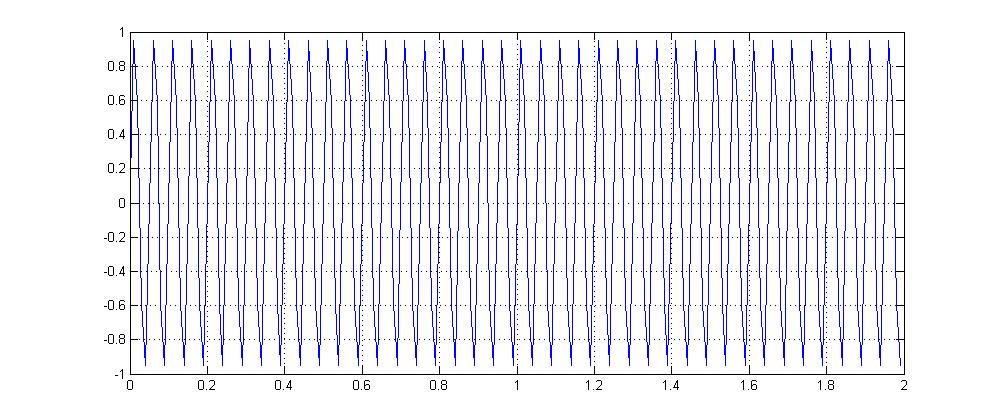
\includegraphics[width=12cm]{1.png} 
\end{figure}
\item Спектр исходного сигнала
\begin{figure}[h]
\centering
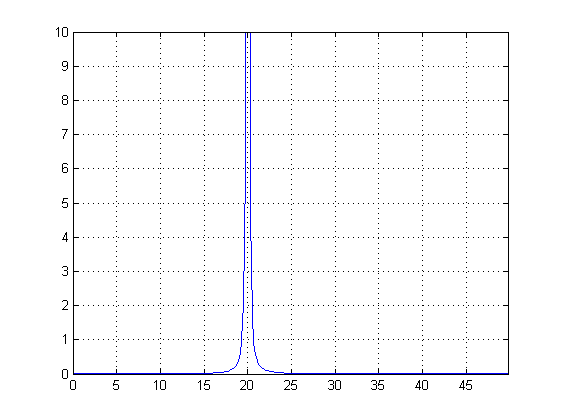
\includegraphics[width=12cm]{2.png} 
\end{figure}
\end{itemize}
\FloatBarrier
\subsubsection{Код MATLAB для зашумленного сигнала}
\%зашумленный сигнал\newline
ynoize = y+ 0.5*rand(size(x));\newline
figure(3)\newline
plot(x(1:200),ynoize(1:200));\newline
grid\newline
\%спектр зашумленного сигнала\newline
spectrum = fft(ynoize,512);\newline
noizespectrum = spectrum.*conj(spectrum)/512;\newline
figure(4)\newline
plot(f, noizespectrum())\newline
axis([0 max(f) 0 10])\newline
grid\newline
\subsubsection{Результаты работы программы}
В результате выполнения программы получились графики временной и частотной характеристик зашумленного синусоидальных сигнала.
\begin{itemize}
\item Зашумленный сигнал
\begin{figure}[h]
\centering
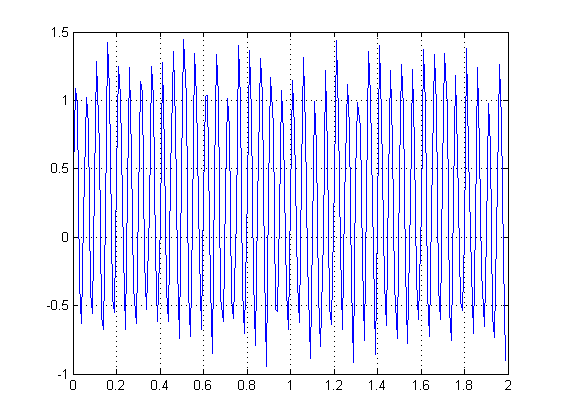
\includegraphics[width=12cm]{3.png} 
\end{figure}
\item Спектр зашумленного сигнала
\begin{figure}[h]
\centering
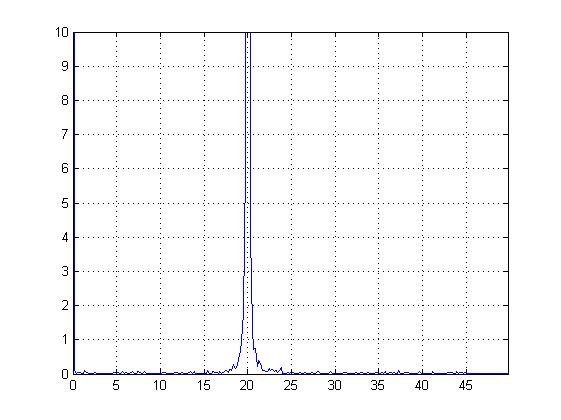
\includegraphics[width=12cm]{4.png} 
\end{figure}
\end{itemize}
\FloatBarrier
\subsection{Вывод}
В данной работе мы построили исходный синусоидальный сигнал, после чего получили его спектр. Далее мы построили зашумленный сигнал и его спектр. По рисункам видно, что спектр зашумленного сигнала очень напонимает спектр исходного сигнала, но является более неровным.
Стоит пояснить возможные расхождения между теоретически ожидаемым и полученным спектром сигнала вследствие дискретности представления сигналов, а также их конечности во времени: конечность сигнала приводит к тому, что спектр сигнала представляет собой sinc(x). Дискретизация сигнала приводит к тому, что в частотной области сигнал повторяется. Разъясним подробнее. В соответствии с теорией мы должны были получить спектр синусоидального сигнала в виде очень короткого импульса бесконечно большой длины. Но на практике на входе мы имеем сигнал ограниченной длины (наш бесконенечный сигнал был умножен на прямоугольное окно), и поэтому его спектр сворачивается со спектром прямоугольного окна.
Так как наш исходный сигнал был дискретизирован, он умножается на решетку дельта-импульсов. Спектром решетки дельта-импульсов является решетка дельта-импульсов. Поэтому спектр нашего сигнала сворачивается с решеткой дельта-импульсов. Так мы получаем спектр в виде нескольких импульсов.

\section{Спектры простых сигналов}
\subsection{Цель работы}
Получить представление о тестовых сигналах во временной и частотной областях. Реализовать операцию свертки сигналов.
\subsection{Постановка задачи}
В командном окне MATLAB и в среде Simulink промоделировать следующие тестовые сигналы:
\paragraph*{-}полигармонический сигнал $y(t)=\sum_{n=0}^{N-1}\cos(nt)$
\paragraph*{-}прямоугольный импульсный сигнал $y(t)=\prod(t,T_i)$
\paragraph*{-} треугольный импульсный сигнал $y(t)=\Delta(t,T_i)$
\paragraph*{}Получить их спектры.
\subsection{Справочные материалы}
В.С. Гутников. Фильтрация измерительных сигналов пп.3-6, 13-14
\subsection{Теория}
\paragraph*{}Спектр - это функция, показывающая зависимость интенсивности различных гармоник в составе сигнала от частоты этих гармоник.Спектр периодического сигнала - это дискретный спектр. Известно, что спектр произведения двух сигналов равен свёртке спектров этих сигналов, а спектр свёртки сигнала равен произведению их спектров.
\paragraph*{}Прямоугольный импульс с единичной амплитудой мы будем обозначать символом $\prod(t,T_i)$.Здесь первый аргумт обозначает положение импульса на горизонтальной оси: середина импульса соответсвует нулю этого аргумента. Второй аргумент - ширину импульса. 
\paragraph*{}Спектр прямоугольного импульса представляется простым выражением:\\*
$\Phi(f)=\int_{\infty}^{- \infty}\prod(t,T_i)e^{-2\pi ft}dt=\int_{\frac{- T_i}{2}}^{\frac{T_i}{2}}e^{-2\pi ft}dt=\frac{\sin(\pi f T_i)}{\pi f}$
\\*
\paragraph*{}Треугольный симметричный импульс, середина которого соответсвует t=0, длительность равна $T_i$, а амплитуда - единице, мы будем обозначать символом $\Delta(t, T_i)$. Такой импульс можно представить в виде свёртки двух одинаковых прямоугольных импульсов длительностью $T_i/2$:\\*
$\Delta(t,T_i)=\frac{2}{T_i}\prod(t,\frac{T_i}{2})*\prod(t,\frac{T_i}{2})$.\\*

\subsection{Полигормонический сигнал}
\subsubsection{Код Matlab}
x = 0:0.01:4*pi;\newline
f=100*(0:255)/512; \newline
figure\newline
y1 = sin(2*pi*x)+sin(2*pi*3*x);\newline
plot(x(1:200),y1(1:200))\newline
grid\newline
figure\newline
s1 = fft(y1,512);\newline
ss1 = s1.*conj(s1)/512;\newline
plot(f,ss1(1:256))\newline
grid \newline
figure\newline
y2 = sin(2*pi*x)+cos(2*pi*x);  \newline
plot(x(1:200),y2(1:200))  \newline 
grid \newline
figure\newline
s2 = fft(y2,512);\newline
ss2 = s2.*conj(s2)/512;\newline
plot(f,ss2(1:256))\newline
grid \newline
\begin{itemize}
\item полигармонический сигнал sin(x)+sin(3x)
\begin{figure}[h]
\centering
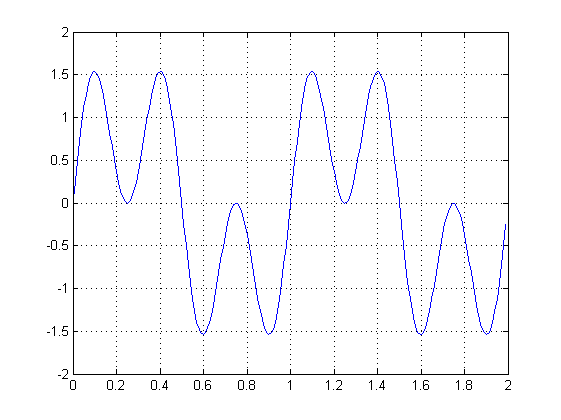
\includegraphics[width=12cm]{5_1.png} 
\end{figure}
\item спектр данного полигармонического сигнала
\begin{figure}[h]
\centering
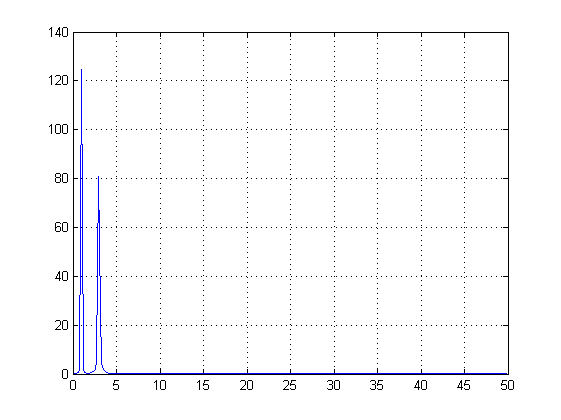
\includegraphics[width=12cm]{5_2.png} 
\end{figure}
\item полигармонический сигнал sin(x)+cos(x)
\begin{figure}[h]
\centering
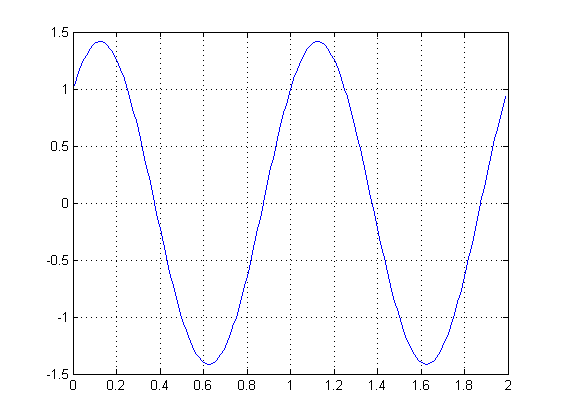
\includegraphics[width=12cm]{12.png} 
\end{figure}
\item спектр данного полигармонического сигнала
\begin{figure}[h]
\centering
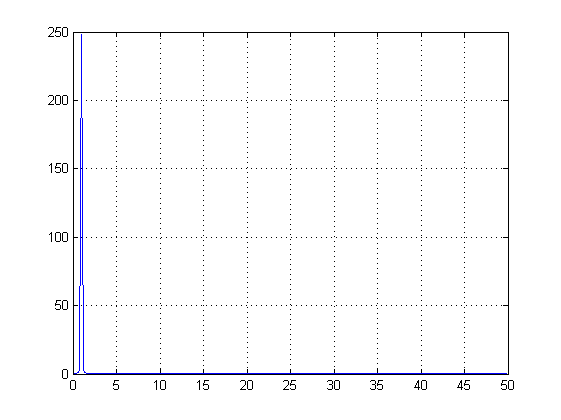
\includegraphics[width=12cm]{11.png} 
\end{figure}
\end{itemize}
\FloatBarrier
\subsubsection{Модуляция в среде Simulink}
\begin{itemize}
\item модель
\begin{figure}[h]
\centering
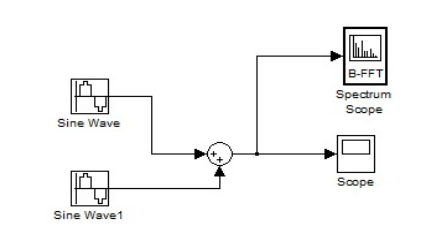
\includegraphics[width=12cm]{sim5_1.png} 
\end{figure}
\item сигнал
\begin{figure}[h]
\centering
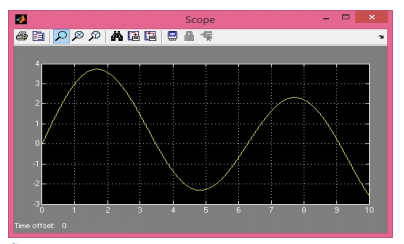
\includegraphics[width=12cm]{sim5_2.png} 
\end{figure}
\item спектр
\begin{figure}[h]
\centering
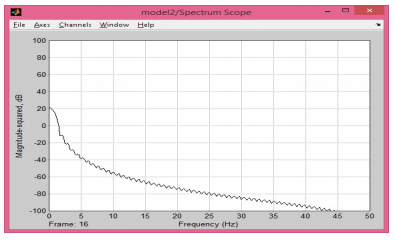
\includegraphics[width=12cm]{sim5_3.png} 
\end{figure}
\end{itemize}
\FloatBarrier
\subsection{Прямоугольный импульсный сигнал}
\subsubsection{Код Matlab}
t=-0.04:1/1000:0.04;\newline
y4=-5*rectpuls(t,0.04);\newline
plot(t,y4);\newline
figure;\newline
spectrum = abs(fft(y4,1024))/1024;\newline
plot(spectrum);\newline
\begin{itemize}
\item Прямоугольный импульсный сигнал
\begin{figure}[h]
\centering
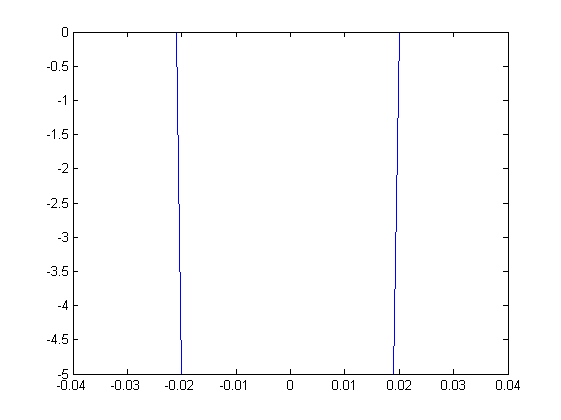
\includegraphics[width=12cm]{5_3.png} 
\end{figure}
\item Спектр прямоугольного сигнала
\begin{figure}[h]
\centering
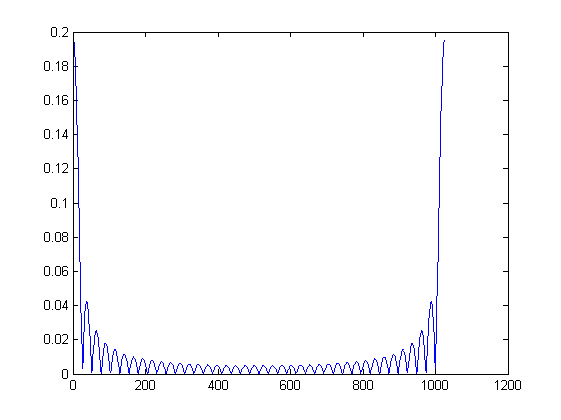
\includegraphics[width=12cm]{5_4.png} 
\end{figure}
\end{itemize}
\FloatBarrier
\subsubsection{Модуляция в среде Simulink}
\begin{itemize}
\item модель
\begin{figure}[h]
\centering
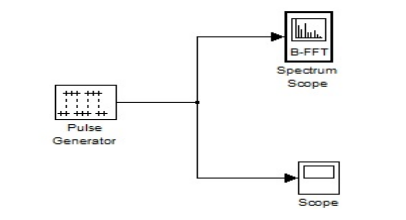
\includegraphics[width=12cm]{sim5_4.png} 
\end{figure}
\item сигнал
\begin{figure}[h]
\centering
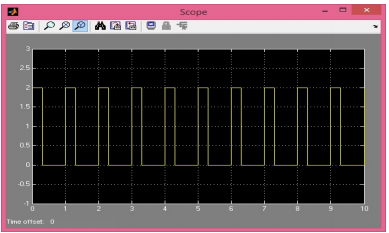
\includegraphics[width=12cm]{sim5_5.png} 
\end{figure}
\item спектр
\begin{figure}[h]
\centering
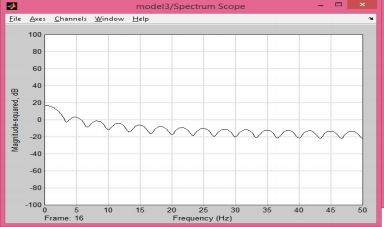
\includegraphics[width=12cm]{sim5_6.png} 
\end{figure}
\end{itemize}
\FloatBarrier
\subsection{Трегольный импульсный сигнал}
\subsubsection{Код Matlab}
t=-0.04:1/1000:0.04;\newline
y4=-5*rectpuls(t,0.02);\newline
y5=-10*rectpuls(t,0.03);\newline
y6= conv(y4,y5);\newline
plot(y6);\newline
figure;\newline
spectrum = abs(fft(y6,1024))/1024;\newline
plot(spectrum);\newline
\begin{itemize}
\item Треугольный импульсный сигнал
\begin{figure}[h]
\centering
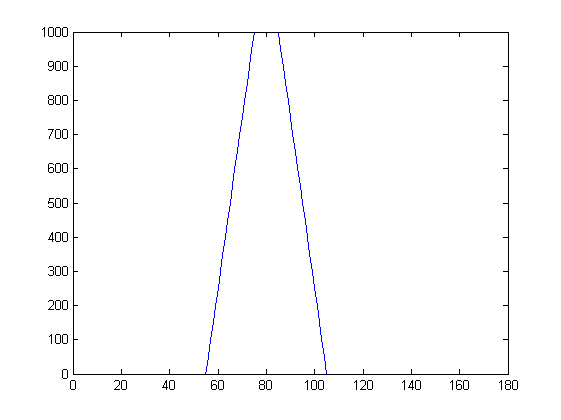
\includegraphics[width=12cm]{5.png} 
\end{figure}
\item Спектр треугольного сигнала
\begin{figure}[h]
\centering
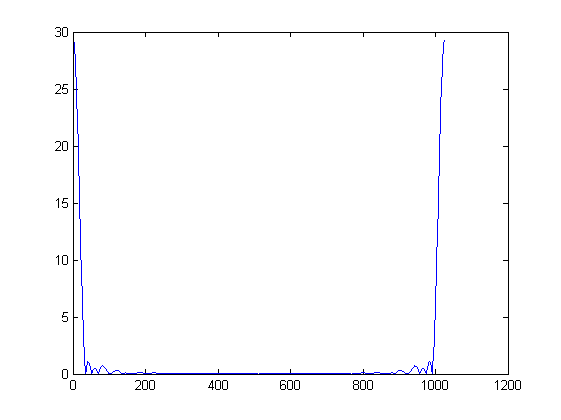
\includegraphics[width=12cm]{6.png} 
\end{figure}
\end{itemize}
\FloatBarrier
\subsubsection{Модуляция в среде Simulink}
\begin{itemize}
\item модель
\begin{figure}[h]
\centering
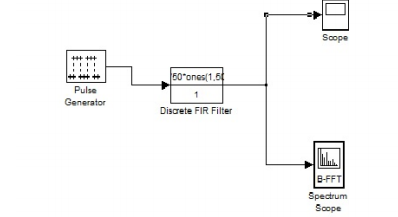
\includegraphics[width=12cm]{sim5_7.png} 
\end{figure}
\item сигнал
\begin{figure}[h]
\centering
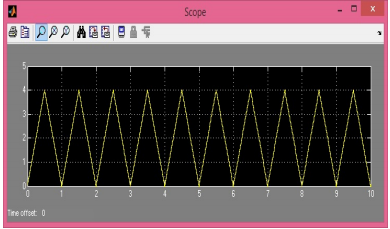
\includegraphics[width=12cm]{sim5_8.png} 
\end{figure}
\item спектр
\begin{figure}[h]
\centering
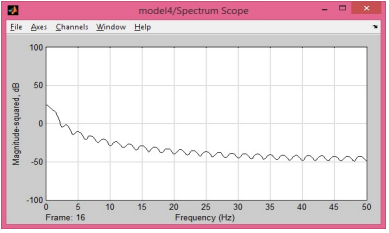
\includegraphics[width=12cm]{sim5_9.png} 
\end{figure}
\end{itemize}
\FloatBarrier
\subsection{Вывод}
В лабораторной работе было проведено моделирование в среде MatLAB и Simulink полигармонического, прямоугольного и треугольного сигналаов. После чего получены их спектры. Для получения сигналов использовались математические формулы данных функций. Треугольный сигнал был получен путем применения операции свертки для двух прямоугольных сигналов. Данная операция осуществляется с помощью специальной функции Matlab. В Simulink для получения генератора треугольного сигнала используется генератор прямоугольных импульсов каскадно с фильтром с прямоугольным окном.\newline
Обоснованием получения треугольного сигнала из свертки двух прямоугольных служит тот факт, что интеграл от произведения двух констант есть линейная функция. График такого преобразования будет представлять две линеные функции, одна из которых имеет положительный коэффициент наклона, а другая отрицательный.

\section{Линейная фильтрация}
\subsection{Цель работы}
Изучить воздействия ФНЧ на тестовый сигнал с шумом. Сгенерировать гармонический сигнал с шумом и синтезировать ФНЧ. Получить сигнал во временной и частотной областях до и после фильтрации.
\subsection{Теоретический материал}
Линейный фильтр — динамическая система, применяющая некий линейный оператор ко входному сигналу для выделения или подавления определённых частот сигнала и других функций по обработке входного сигнала, т.е. это устройство целенаправленным образом изменяющее спектр сигнала.\\*
Фильтры бывают следующих видов: фильтры нижних частот(ФНЧ) -  пропускают низкочастотные состовляющие спектра и задерживают высокочастотные; фильтры верхних частот(ФВЧ) -  пропускают только высочастотные состовляющие, фильтры полосно пропускающие(ФПП)  - пропускают состовляющие сигнала в определенной полосе частот и фильтры полосно-заграждающие(ФПЗ) - пропускают все состовляющие спектра кроме заданной полосы.\\*
Фильтры с конечной импульсной характеристикой (КИХ-фильтры) - их импульсная характеристика ограничена во времени. Фильтры с бесконечной импульсной характеристикой (БИХ-фильтры) - их импульсная характеристика, хоть и затухает во времени, теоретиески неограничена во времени.
\subsection{Ход работы}
В данной работе в качестве ФНЧ используем фильтр Баттерворта, который синтезируем с помощью функции Matlab - BUTTER.Фильтр Баттерворта является БИХ фильтром. Порядок фильтра равен 16.\\*
 В командном окне Matlab сгенерируем гармонический сигнал без шума и с шумом, а также спектры сигнала с шумом и без шума. В результате код Matlabа будет выглядеть так:
\begin{verbatim}
x = 0:0.01:4*pi;
f=100*(0:255)/512;
figure
noise=rand(size(x));
y = sin(2*pi*x);
y_noisy = y+0.3*noise;

%Построение сигнала без шума:
plot(x(1:200),y(1:200))
grid

%Построение сигнала с шумом:
plot(x(1:200),y_noisy(1:200))
grid

%синтез ФНЧ Баттерворта
[B,A] = butter(16,0.99);
B=B./sum(B);
A=A./sum(A);
%обработка сигнала ФНЧ
figure
y_filtered = conv(y_noisy,[B,A]);

%Построение сигнала после прохождения через фильтр:
plot(x(1:200),y_filtered(1:200))
grid
figure
%Построение спектра сигнала с шумом
noisy_spectrum = fft(y_noisy,512);
norm_noisy_spectrum = noisy_spectrum.*conj(noisy_spectrum)/512;

%Построение нормирова спектра сигнала с шумом:
plot(f,norm_noisy_spectrum(1:256))
axis([0 max(f) 0 2])
grid
figure

%Спектр отфильтрованного сигнала
spectrum = fft(y_filtered,512);
norm_filtered_spectrum=spectrum.*conj(spectrum)/512;
%Построение нормированого отфильтрованного спектра:
plot(f,norm_filtered_spectrum(1:256))
axis([0 max(f) 0 2])
grid
\end{verbatim}
Результаты работы программы на рисунке.
\begin{figure}[H]
\begin{minipage}[h]{0.6\linewidth}
\center{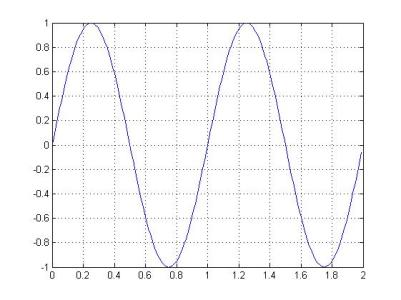
\includegraphics[width=1\linewidth]{im1}} a) \\
\end{minipage}
\vfill
\begin{minipage}[h]{0.6\linewidth}
\center{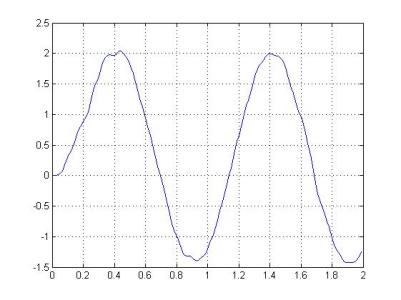
\includegraphics[width=1\linewidth]{im2}} \\б)
\end{minipage}
\hfill
\begin{minipage}[h]{0.6\linewidth}
\center{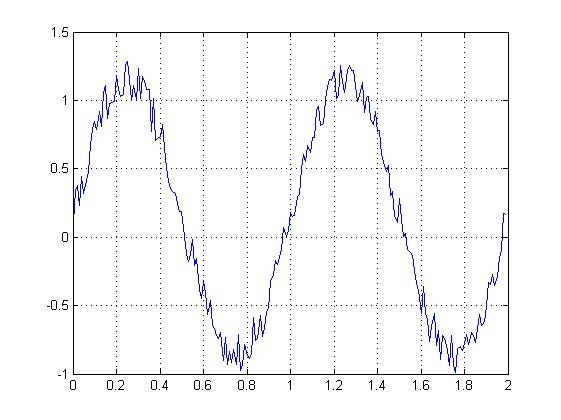
\includegraphics[width=1\linewidth]{im56}} в) \\
\end{minipage}

\vfill
\begin{minipage}[h]{0.6\linewidth}
\center{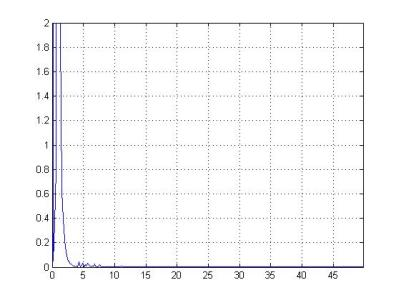
\includegraphics[width=1\linewidth]{im4}} г) \\
\end{minipage}
\hfill
\begin{minipage}[h]{0.6\linewidth}
\center{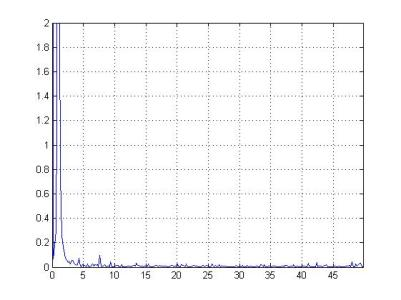
\includegraphics[width=1\linewidth]{im3}} д) \\
\end{minipage}
\caption{Линейная фильтрация в Matlab: a) Сигнал без шума, б)
Сигнал после фильтрации, в)Сигнал с шумом, г)Спектр сигнала после фильтрации, д)Спектр сигнала с шумом.}
\label{ris:experimentalcorrelationsignals}
\end{figure}
\FloatBarrier
\subsection{Моделирование в Simulink}
Для создания модели в Simulink используем блок Discrete FIR Filter раздела Discrete главной библиотеки и блок Digital Filter design из Signal Processing Blockset/Filtering/Filter Designs. Результаты моделирование в Simulink на рисунке.
\begin{figure}[H]
\begin{minipage}[h]{0.6\linewidth}
\center{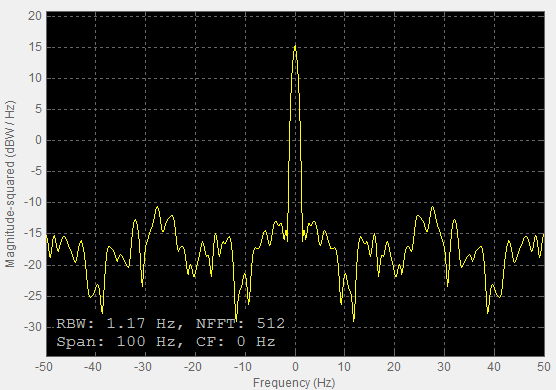
\includegraphics[width=1\linewidth]{im7}} a) \\
\end{minipage}
\hfill
\begin{minipage}[h]{0.6\linewidth}
\center{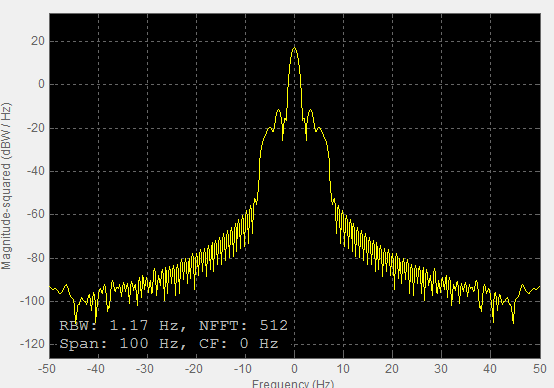
\includegraphics[width=1\linewidth]{im6}} \\б)
\end{minipage}
\vfill
\begin{minipage}[h]{0.6\linewidth}
\center{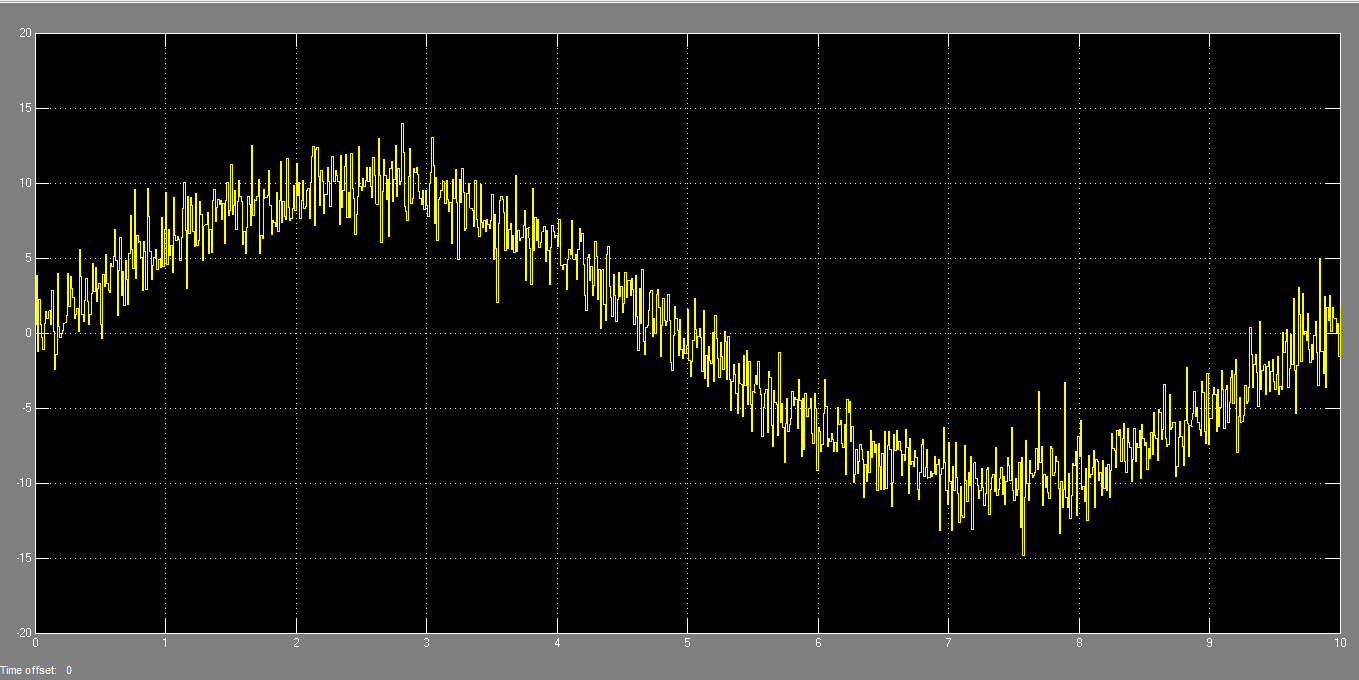
\includegraphics[width=1\linewidth]{im8}} в) \\
\end{minipage}
\hfill
\begin{minipage}[h]{0.6\linewidth}
\center{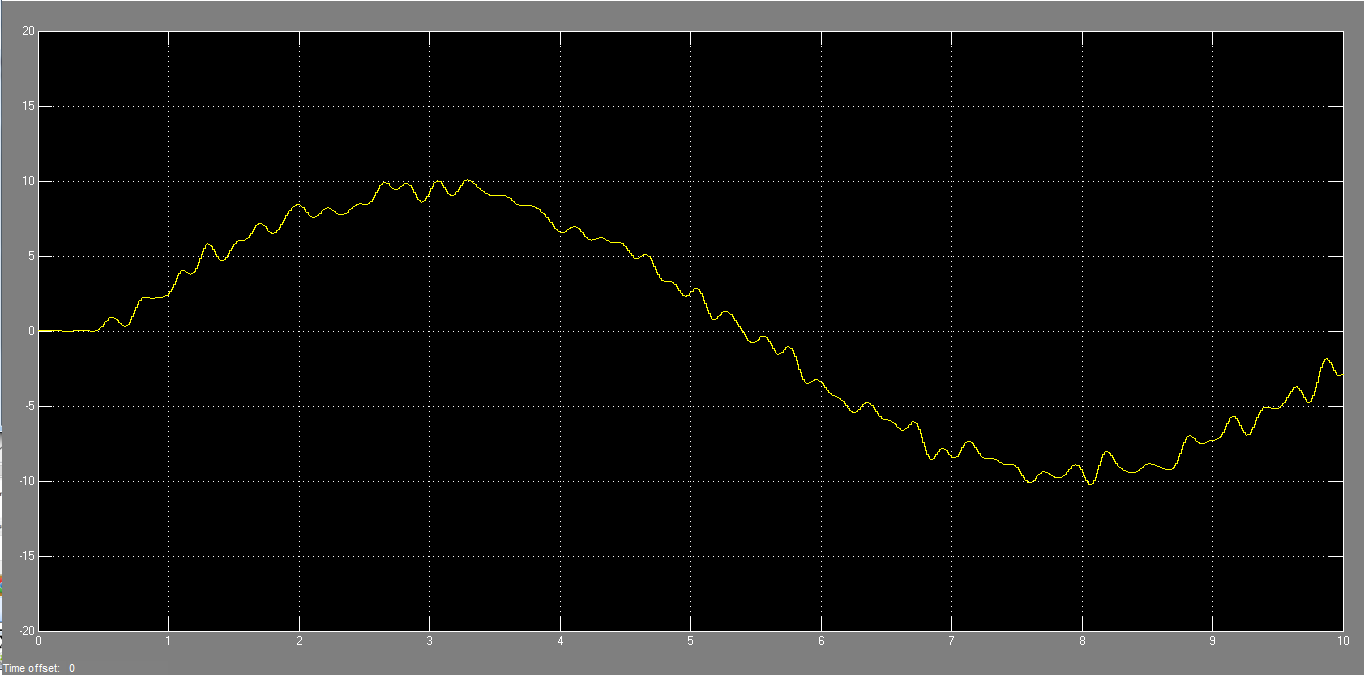
\includegraphics[width=1\linewidth]{im9}} г) \\
\end{minipage}
\hfill
\begin{minipage}[h]{0.6\linewidth}
\center{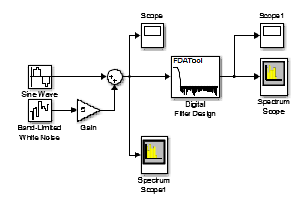
\includegraphics[width=1\linewidth]{im5}} д) \\
\end{minipage}
\caption{Линейная фильтрация в Simulink: a) Спектр до фильтрации, б)
Спектр после фильтрации, в)Сигнал до фильтрации, г)Сигнал после фильтрации, д) Схема модели.}
\label{ris:experimentalcorrelationsignals}
\end{figure}
\FloatBarrier
\subsection{Вывод}
Фильтр нижних частот — это фильтр, который  эффективно пропускает частотный спектр сигнала ниже некоторой частоты  и подавляет частоты сигнала выше этой частоты. Степень подавления каждой частоты зависит от вида и порядка фильтра. В лабораторной работе было произведено удаление шума линейным фильтром. Отметим, что на практике фильтрация только подавляет шум, для полного удаления шума необходимо использовать идеальный фильтр с прямоугольным окном, которого на практике не существует.  Также заметим, что линейный фильтр подавляет все сигналы, находящиеся в его полосе задержания и не изменяет сигналы из полосы пропускания, и поэтому не может удалить шум, который попал в его полосу пропускания. 
\section{Аналоговая модуляция}
\subsection{Цель работы}
Изучить процесс амплитудной модуляции/демодуляции сигнала.
\subsection{Алгоритм работы}
\begin{itemize}
\item Сгенерировать однотональный сигнал низкой частоты.
\item Выполнить амплитудную модуляцию (АМ) сигнала по закону 
\begin{displaymath}
u(t)=(1+M*U_{m}*cos(\Omega*t))*cos(\omega_{0}*t+\phi_{0})\newline
\end{displaymath}
  для различных значений глубины модуляции M.
\item Получить спектр модулированного сигнала.
\item Выполнить модуляцию с подавлением несущей: 
\begin{equation}
	u(t) = MU_m cos(\omega t)cos(\omega_0 t+\phi_0).
          \end{equation}
Получить спектр.
\item Выполнить однополосную модуляцию:
\begin{equation}
  u(t) = U_m cos(\omega t)cos(\omega_0 t+\phi_0)+\frac{U_m}{2}\sum_{n=1}^N M_n (cos(\omega_0 + \Omega_n )t + \phi_0 + \Phi_n ),
  \end{equation}
положив n = 1.
\item Выполить синхронное детектирование и получить исходный однополосный сигнал.
\item Рассчитать КПД модуляции:
\begin{equation}
					\eta_A M = \frac{U_m ^2 M^2 /4}{P_U} = \frac{M^2}{M^2 + 2}.
				\end{equation}
\end{itemize}
\subsection{Теоретические сведения}
Модуляция - это процесс, при котором высокочастотная волна используется для переноса низкочастотной волны. Другими словами, перенос спектра сигналов из низкочастотной области в выделенную для их передачи область высоких частот и выполняется операцией модуляции.\\*
При амплитудной модуляции в соответствии с модулирующим сигналом изменяется амплитуда несущего колебания. АМ соответствует переносу информации s(t)=>U(t) при постоянных значениях параметров несущей частоты w и f (частоты и фазы). АМ – сигнал представляет собой произведение информационной огибающей U(t)  и гармонического колебания ее заполнения с более высокими частотами.
Форма записи амплитудно-модулированного сигнала:
\begin{displaymath}
u(t)=(1+M*U_{m}*cos(\Omega*t))*cos(\omega_{0}*t+\phi_{0})\newline
\end{displaymath}
, где U – постоянная амплитуда несущего колебания при отсутствии входного (модулирующего) сигнала s(t), M  – коэффициент амплитудной модуляции. Значение  M характеризует глубину амплитудной модуляции. В зависимости от значения  M различают нормальную модуляцию ( M<1 ), глубокую модуляцию ( M=1 ) и перемодуляцию ( M>1 ).\\*
Получим спектр модулированного сигнала:\\*
$$ u(t) = U_m cos(\omega_0 t) + (U_m * M/2)cos[(\omega_0 + \Omega)t] + (U_m * M/2)cos[(\omega_0 - \Omega)t] $$
КПД амплитудной модуляции равен 
\begin{displaymath}
\eta_{A}*M=\frac{M^{2}}{M^{2}+2}
\end{displaymath}
Как видно, основная доля мощности АМ – сигнала приходится на несущую частоту. При балансной модуляции (с подавлением несущей) производится перемножение двух сигналов – модулирующего и несущего, при котором происходит подавление несущего колебания, соответственно, КПД модуляции становится равным 100%. Так, для однотонального сигнала (без учета начальных фаз колебаний) при 
\begin{displaymath}
u(t)=M*cos(\Omega*t))
\end{displaymath}  имеем
\begin{displaymath}
u(t)=M*U_{m}*cos(\Omega*t)*cos(\omega_{0}*t)=U_{m}*\frac{M}{2}*(cos((\omega_{0}+\Omega)*t)+cos((\omega_{0}-\Omega)*t)))
\end{displaymath}
 , т.е. два одинаковых по амплитуде гармонических сигнала с верхней и нижней боковыми частотами. По существу, однотональный модулирующий сигнал переносится на две высокие частоты.
\subsection{Код MATLAB для п.1-3}
f0=3; частота сигнала \newline
fd=150; частота дискретизации\newline
fc=30; частота несущего колебания\newline
x=0:0.01:4*pi;\newline
y=0.5*sin(2*pi*f0*x);\newline
plot(x(1:200),y(1:200))\newline
grid;\newline
figure\newline
M1=0.3; \newline
M2=1;\newline
M3=1.3;\newline
t=0:0.001:10;\newline
Um=0.5;\newline
f=100*(0:255)/512;\newline
u1=(1+Um*M1*cos(f0*t)).*cos(fc*t); модулированный сигнал\newline
plot(t,u1)\newline
figure\newline
s1=fft(u1,512); спектр модулированного сигнала\newline
ss1=s1.*conj(s1)/512;\newline
plot(f,ss1(1:256));\newline
figure\newline
u2=Um*(1+M2*cos(f0*t)).*cos(fc*t);\newline
plot(t,u2)\newline
figure\newline
s2=fft(u2,512);\newline
ss2=s2.*conj(s2)/512;\newline
plot(f,ss2(1:256));\newline
figure\newline
u3=Um*(1+M3*cos(f0*t)).*cos(fc*t);\newline
plot(t,u3)\newline
figure\newline
s3=fft(u3,512);\newline
ss3=s3.*conj(s3)/512;\newline
plot(f,ss3(1:256));\newline
\begin{figure}[h]
\centering
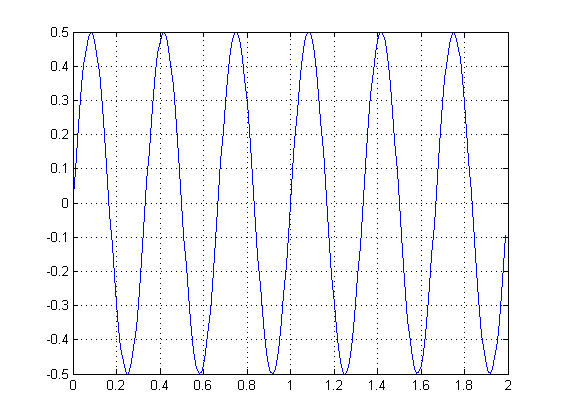
\includegraphics[width=12cm]{am1_1.png} 
Исходный низкочастотный сигнал
\end{figure}
\FloatBarrier
\begin{figure}[H]
\begin{minipage}[h]{0.6\linewidth}
\center{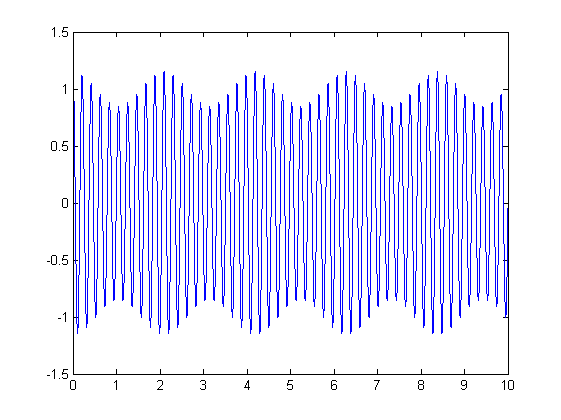
\includegraphics[width=1\linewidth]{am1_2}} а)\\
\end{minipage}
\hfill
\begin{minipage}[h]{0.6\linewidth}
\center{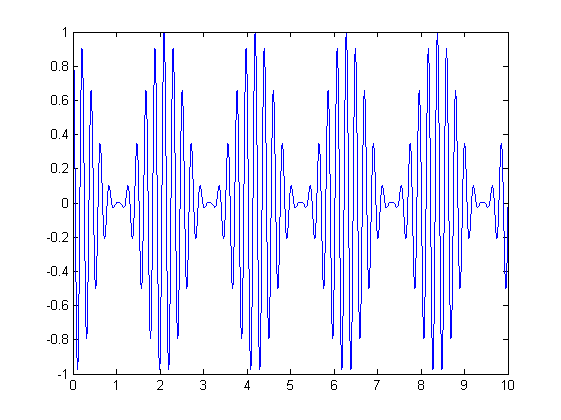
\includegraphics[width=1\linewidth]{am1_4}} б) \\
\end{minipage}
\hfill
\begin{minipage}[h]{0.6\linewidth}
\center{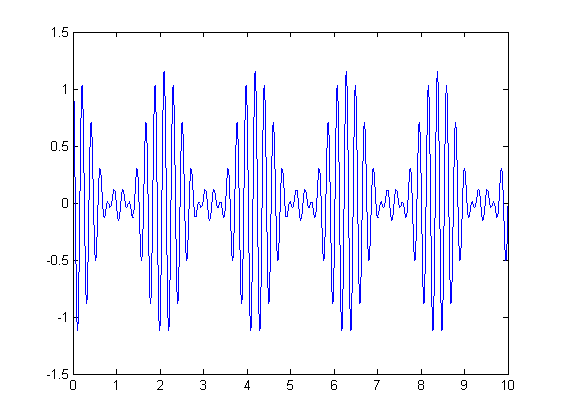
\includegraphics[width=1\linewidth]{am1_6}} в) \\
\end{minipage}
\hfill
\begin{minipage}[h]{0.6\linewidth}
\center{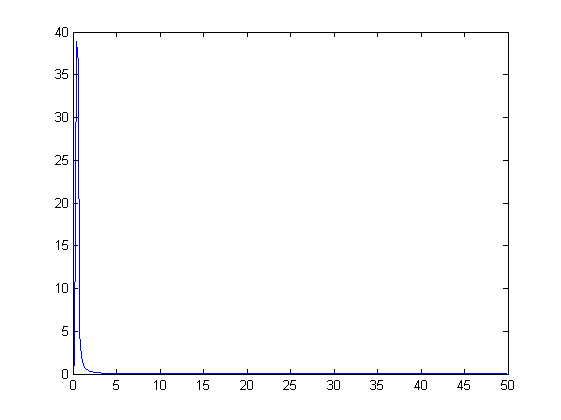
\includegraphics[width=1\linewidth]{am1_5}} г) \\
\end{minipage}
\begin{minipage}[h]{0.6\linewidth}
\center{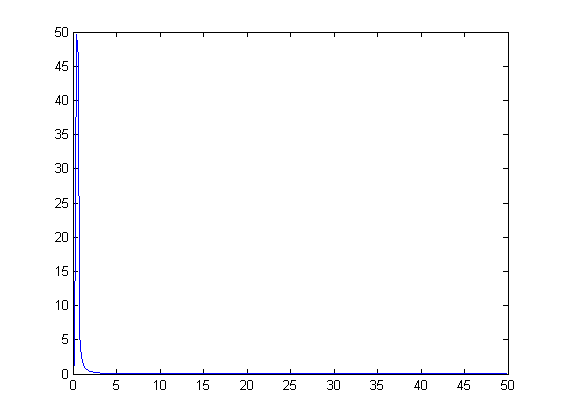
\includegraphics[width=1\linewidth]{am1_7}} д) \\
\end{minipage}
\begin{minipage}[h]{0.6\linewidth}
\center{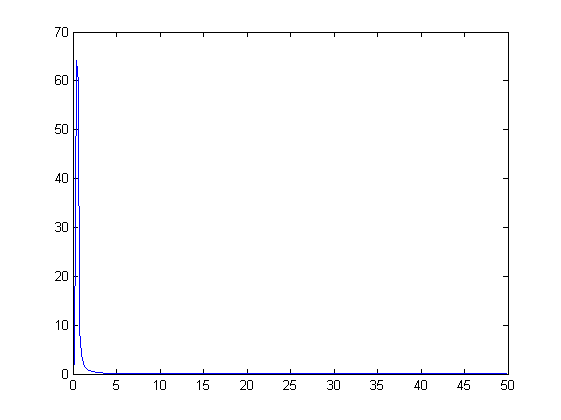
\includegraphics[width=1\linewidth]{am1_3}} е) \\
\end{minipage}
\caption{Линейная фильтрация в Simulink: а)
АМ при степени глубины=0.3, б)АМ при степени глубины=1, в)АМ при степени глубины=1.3, г) Спектр модулированного сигнала при степени глубины=0.3, д) Спектр модулированного сигнала при степени глубины=1, е) Спектр модулированного сигнала при степени глубины=1.3.}
\label{ris:experimentalcorrelationsignals}
\end{figure}
\FloatBarrier
\subsection{Код MATLAB для п.4}
 plot(x(1:200),y(1:200)) исходный сигнал\newline
grid;\newline
figure\newline
u4=Um*M1*cos(f0*t).*cos(fc*t); модуляция с подавлением несущей\newline
plot(t,u4) \newline
figure\newline
s4=fft(u4,512);\newline
ss4=s4.*conj(s4)/512;\newline
plot(f,ss4(1:256));
figure\newline
plot(t,YY);\newline
\begin{figure}[H]
\begin{minipage}[h]{0.6\linewidth}
\center{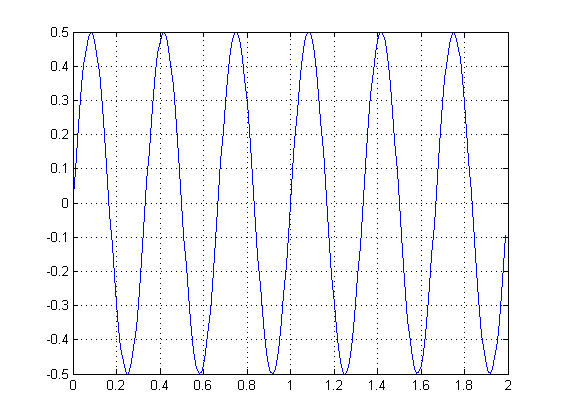
\includegraphics[width=1\linewidth]{am1_1}} а)\\
\end{minipage}
\hfill
\begin{minipage}[h]{0.6\linewidth}
\center{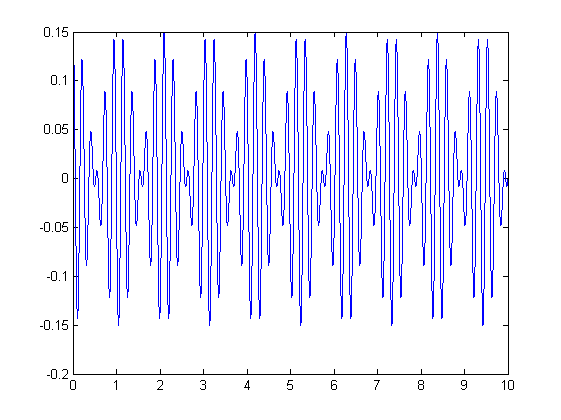
\includegraphics[width=1\linewidth]{am2_2}} б) \\
\end{minipage}
\hfill
\begin{minipage}[h]{0.6\linewidth}
\center{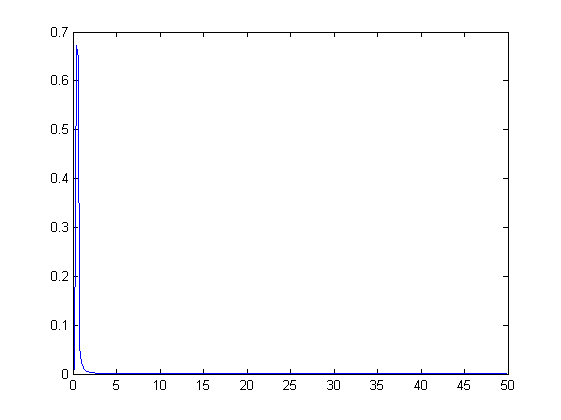
\includegraphics[width=1\linewidth]{am2_3}} в) \\
\end{minipage}
\hfill
\caption{Линейная фильтрация в Simulink: а)
Исходный низкочастотный сигнал, б)Модулированный сигнал с подавлением несущей, в) Спектр модулированного сигнала с подавлением несущей.}
\label{ris:experimentalcorrelationsignals}
\end{figure}
\FloatBarrier
\subsection{Код MATLAB для п.5}
 x=0:0.01:4*pi;\newline
y=sin(2*pi*2*x); \newline
plot(x(1:200),y(1:200),'r')\newline 
t=0:0.001:10;\newline
u2=(1+1*cos(2*t)).*cos(20*t);\newline
s2=fft(u2,512);\newline
yy=u2.*cos(20*t);\newline
plot(t,yy,'r');\newline
ss=fft(yy,512);\newline
sss=ss.*conj(ss)/512;\newline
plot(f,sss(1:256),'r');\newline
\begin{figure}[H]
\begin{minipage}[h]{0.8\linewidth}
\center{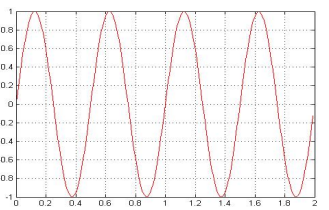
\includegraphics[width=1\linewidth]{am3_3}} а)\\
\end{minipage}
\vfill
\begin{minipage}[h]{0.8\linewidth}
\center{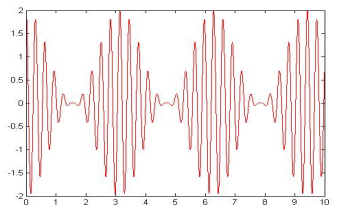
\includegraphics[width=1\linewidth]{am3_1}} б) \\
\end{minipage}
\vfill
\begin{minipage}[h]{0.8\linewidth}
\center{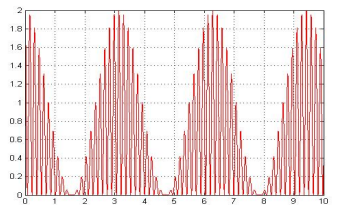
\includegraphics[width=1\linewidth]{am3_2}} б) \\
\end{minipage}
\vfill
\caption{Линейная фильтрация в Simulink: а)
Исходный сигнал, б)Модулированный сигнал, в)Сигнал после выполнения синхронного детектирования.}
\label{ris:experimentalcorrelationsignals}
\end{figure}
\FloatBarrier
\subsection{Код MATLAB для п.6}
Найдем КПД модуляции по формуле
\begin{displaymath}
\eta_{A}*M=\frac{M^{2}}{M^{2}+2}
\end{displaymath}
\begin{center}
M=0.3; КПД=0.14\newline
M=1; КПД=0.3(3)\newline
M=1.3; КПД=0.35\newline
\end{center}
\subsection{Вывод}
В результате выполнения лабораторной работы был сгенерирован однотональный сигнал низкой частоты, выполнена АМ сигнала и получен спектр модулированного сигнала, выполнена БАМ и однополосная АМ и получены их спектры. Далее произведено синхронное детектирование и получен исходный однополосный сигнал. Рассчитан КПД модуляции.\\*
АМ - сигнал представляет собой произведение информационной огибающей U(t) и гармонического колебания ее заполнения с более высокими частотами. Значение М должно находиться в пределах от 0 до 1 для всех гармоник модулирующего сигнала. Малую глубину модуляции (M<1) применять неце-
лесообразно, т.к. при этом мощность передаваемого информационного сигнала будет много меньше мощности несущего колебания, и мощность
передатчика используется неэкономично.\\*
В настоящее время амплитудная модуляция применяется редко (для радиовещания и для передачи изображения в телевизионном вещании) из-за низкого КПД использования энергии модулированных сигналов.\\*
Для однотональной модуляции начальная фаза модулирующего колебания для верхней боковой частоты складывается с начальной фазой несущей, для нижней – вычитаются из фазы несущей. Как в случае с обычной АМ, так и в случае АМ с подавленной несущей ширина спектра АМ-сигнала  в два раза больше, чем у модулирующего сигнала. При балансной амплитудной модуляции производится перемножение двух сигналов – модулирующего и несущего, при котором происходит подавление несущего колебания, и тогда КПД модуляции становится равным 100.\\*
Синхронное детектирование - это один из способов демодуляции АМ-сигнала. Его суть состоит в умножении частоты сигнала на опорное колебание с несущей частотой. В результате умножения получаем два слагаемых: искомая амплитуда и АМ-сигнал с несущей частотой 2wo, который удаляется в результате пропускания сигнала через ФНЧ. 

\section{Частотная и фазовая модуляция}

\subsection{Цель работы}
Изучение частотной и фазовой модуляции/демодуляции сигнала.

\subsection{Постановка задачи}
	\begin{enumerate}
		\item Сгенерировать однотоальный сигнал низкой частоты.
		\item Выполнить фазовую модуляцию/демодуляцию сигнала по закону
				\begin{equation}
					u(t) = U_m cos(\Omega t + ks(t)),
				\end{equation}
		используюя встроенную функцию MatLab pmmod, pmdemod.
		\item Получить спектр модулированного сигнала.
		\item Выполнить частотню модуляцию/демодуляцию по закону
				\begin{equation}
					u(t) = U_m cos(\omega_0 t + k \int_0^t s(t) dt + \phi_0),
				\end{equation}
		используюя встроенные функции MatLab fmmod, fmdemod.
	\end{enumerate}

\subsection{Справочные материалы}
Н.В. Богач и др. Обработка сигналов в информационных системах, с. 118-125, 127-133.

\subsection{Теоретический материал}
Фазовая модуляция – процесс изменения мгновенной фазы несущего колебания пропорционально изменению непрерывного информационного сигнала, т.е. информациооный сигнал управляет фазой несущего колебания (амплитуда и частота несущего колебания остаются постоянными). Фазомодулированный сигнал s(t) имеет следующий вид:
	\begin{equation}
	s(t) = g(t) \sin[2 \pi f_c t + \varphi(t)],
	\end{equation}
где g(t) — огибающая сигнала; $\varphi(t)$ является модулирующим сигналом; $f_c$ — частота несущего сигнала; t — время. \\*
Частотная модуляция - это процесс изменения мгновенной частоты несущего колебания в соответствии и изменением информационного сигнала, т.е. информациооный сигнал управляет частотой несущего колебания (амплитуда и фаза несущего колебания остаются постоянными). \\*
По характеристикам фазовая модуляция близка к частотной модуляции. В случае синусоидального модулирующего (информационного) сигнала, результаты частотной и фазовой модуляции совпадают.\\*

\subsection{Ход работы}
\begin{enumerate}
\item Сгенерирован однотональнаый сигнал низкой частоты. Выполнена фазовая модуляция/демодуляция сигнала.Получен спектр модулированного сигнала.
Код в командном окне MATLAB:
\\
x = 0:(1/(8*pi)):2*pi;
\\
y = sin(pi*x+pi/2); 
\\
y1=pmmod(y, 5, 50, 1, 3*pi/2); Фазовая модуляция
\\
y2=pmdemod(y1, 5, 50, 1, 3*pi/2); Фазовая демодуляция
\\
\\
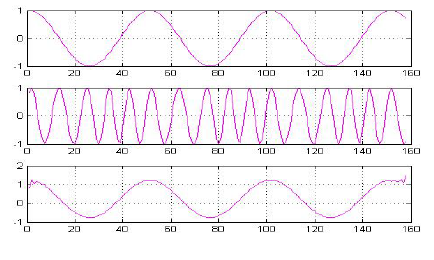
\includegraphics[width=6in,height=80mm]{r81}
\\
Исходный, модулированный, демодулированный сигналы
\\
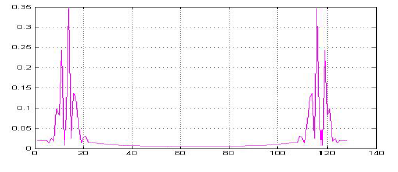
\includegraphics[width=4in,height=40mm]{r82}
\\
Спектр
\\
\item Выполнена частотная модуляция/демодуляция сигнала. Получен спектр модулированного сигнала.
\\Код в командном окне MATLAB:
\\
x = 0:(1/(8*pi)):2*pi;
\\
y = sin(pi*x+pi/2); 
\\
z1=fmmod(y, 5, 50, 1, 3*pi/2); Частотная модуляция
\\
z2=fmdemod (z1, 5, 50, 1, 3*pi/2); Частотная демодуляция
\\
\\
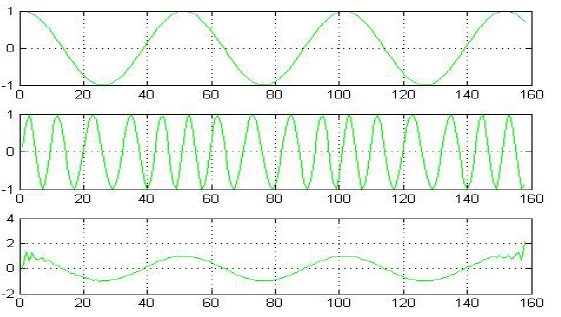
\includegraphics[width=6in,height=80mm]{r83}
\\
Исходный, модулированный, демодулированный сигналы
\\
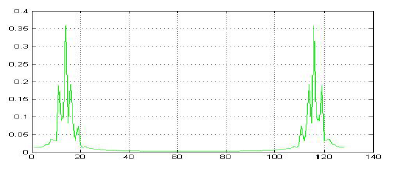
\includegraphics[width=4in,height=40mm]{r84}
\\
Спектр
\\
\item Фазовая модуляци в среде Multisim
\\
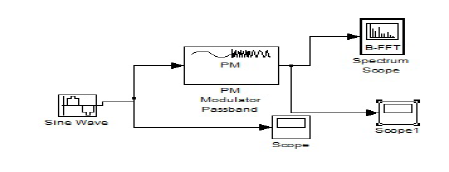
\includegraphics[width=4in,height=40mm]{r85}
\\
Схема simulink
\\
\\
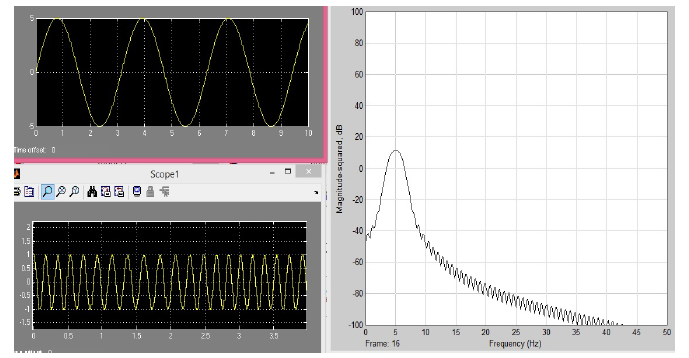
\includegraphics[width=6in,height=80mm]{r86}
\\
Исходный сигнал, модулированный сигнал, спектр модулированного сигнала
\\
\item Частотная модуляци в среде Multisim
\\
\includegraphics[width=4in,height=40mm]{r87}
\\
Схема simulink
\\
\\
\includegraphics[width=6in,height=80mm]{r88}
\\
Исходный сигнал, модулированный сигнал, спектр модулированного сигнала
\\
\item Блок фазовой автоподстройки частоты(ФАПЧ)
\\
\includegraphics[width=4in,height=40mm]{r89}
\\
Схема simulink
\\
\\
\includegraphics[width=4in,height=40mm]{r90}
\\
Исходный сигнал
\\
\\
\includegraphics[width=4in,height=40mm]{r91}
\\
Модулированный сигнал
\\
\\
\includegraphics[width=4in,height=40mm]{r92}
\\
Сигнал на выходе ФНЧ
\\
\\
\includegraphics[width=4in,height=40mm]{r93}
\\
Сигнал на выходе фазового детектора
\\
\\
\includegraphics[width=4in,height=40mm]{r94}
\\
Сигнал на выходе ГУН(генератор, управляемый напряжением)
\\
\\
\end{enumerate}

\subsection{Выводы}
В результате выполнения данной работы были выполнены частотная и фазовая модуляция/демодуляция, а также чатотная демодуляция с  помощью блока захвата фазы. Сделаем вывод, что частотная и фазовая модуляция очень тесно взаимосвязаны, поскольку обе они влияют на аргумент функции cos. Поэтому эти два вида модуляции имеют общее название — угловая модуляция.Сигнал с угловой модуляцией имеет вид колебания, начальная фаза которого зависит от времени:
	\begin{equation}
	s_(t) = A_0 cos(\omega0 t + j(t)).
	\end{equation}
В случае фазовой модуляции частота несущей зависит от производной модулируемого сигнала, а в случае частотной - от самого его значения.\\*
Схема ФАПЧ позволяет обеспечить точную настройку, частотную селекцию и фильтрацию без использования громоздких элементов фильтров, используемых в схемах детектирования. ФАПЧ представляет собой систему управления с петлей обратной связи, в которой параметрами регулирования 
являются частота или фаза сигнала. При подаче на вход схемы сигнала с угловой модуляцией на выходе ФНЧ после захвата частоты и фазы формируется сигнал, пропорциональный модулирующему сигналу, что позволяет применять схему ФАПЧ для демодуляции.Для демодуляции использовалась петля ФАПЧ, состоящая из перемножителя (используемого в качестве фазового детектора), фильтра нижних частот и генератора, управляемого напряжением (ГУН). Если собственная частота ГУН f0 достаточно близка к частоте внешнего опорного сигнала fi, то под действием обратной связи в схеме ФАПЧ ГУН синхронизируется, то есть захватывает внешний входной сигнал. Поэтому выходная частота ГУН – это сумма или разность его собственной частоты и разницы между внешней опорной частотой и собственной частотой ГУН.

\section{Цифровая модуляция}
\subsection{Цель работы}
Изучение методов модуляции цифровых сигналов и сравнение их свойств. 
\subsection{Алгоритм работы}
\begin{itemize}
\item Получить сигналы BPSK, PSK, OQPSK, genQAM, MSK, M-FSK модуляторов 
\item Построить их сигнальные созвездия. 
\item Провести сравнение изученных методов модуляции цифровых сигналов. 
\end{itemize}
\subsection{Теоретическая часть}
В настоящее время все большая часть информации, передаваемой по разнообразным каналам связи, существует в цифровом виде. Это означает, что передаётся последовательность целых чисел, которые могут принимать значения из некоторого фиксированного конечного 
множества. Эти числа, называемые символами (symbol), поступают от источника информации с периодом T, а частота, соответствующая этому периоду, называется символьной скоростью (symbol rate): fT = 1/T.  
Последовательность передаваемых символов является дискретным сигналом. Поскольку символы принимают значения из конечного множества, этот сигнал является и квантованным, то есть его можно назвать цифровым сигналом. В данной работе рассматриваться вопросы, связанные с преобразованием этого цифрового сигнала в аналоговый 
модулированный сигнал. 
Типичный подход при осуществлении передачи дискретной последовательности символов состоит в следующем. Каждому из возможных значений символа сопоставляется некоторый набор параметров несущего колебания. Эти параметры поддерживаются постоянными в течение 
интервала T, то есть до прихода следующего символа. Фактически это означает преобразование последовательности чисел {nk} в ступенчатый сигнал sn(t) : 
sn(t) = f(nk), kT <= t < (k + 1)T. 
Здесь f — некоторая функция преобразования. Полученный сигнал sn(t)далее используется в качестве модулирующего сигнала обычным способом. 
Такой способ модуляции, когда параметры несущего колебания меняются скачкообразно, называется манипуляцией (keying). В зависимости от того, какие именно параметры изменяются, различают амплитудную (АМн),фазовую (ФМн), частотную (ЧМн) и квадратурную (КАМн) 
манипуляцию. 
Цифровая модуляция и демодуляция включают в себя две стадии. При модуляции цифровое сообщение сначала преобразуется в аналоговый модулирующий сигнал с помощью функции modmap, а затем осуществляется аналоговая модуляция. При демодуляции сначала получается аналоговый демодулированный сигнал, а затем он преобразуется в цифровое сообщение с помощью функции demodmap.  
Функция randerr предназначена для формирования ошибок в цифровом сигнале. Она дает матрицу, в каждой строке которой имеется заданное число случайно расположенных ненулевых элементов. Для оценки помехоустойчивости системы связи необходимо произвести сравнение 
исходного (передаваемого) сообщения с сообщением, полученным в результате приема, и определить число ошибок, возникших в процессе передачи, а также вероятность ошибки. Эти действия выполняются функциями symerr и biterr, первая из которых подсчитывает число 
несовпадающих символах в двух сообщениях, а вторая — число несовпадающих битов в двоичных представлениях этих символов. Кроме числа ошибок, обе функции могут возвращать долю ошибок в общем числе символов (битов) и индикаторы мест возникновения ошибок. 
Последние две функции данной группы предназначены для графического отображения сигналов с квадратурной манипуляцией. Функция eyediagram выводит так называемую глазковую диаграмму, а функция scatterplot — диаграмму рассеяния. 
Аналоговый несущий сигнал модулируется цифровым битовым потоком.
Существуют три фундаментальных типа цифровой модуляции (или шифтинга) и один гибридный:
\begin{enumerate}
    \item ASK – Amplitude shift keying (Амплитудная двоичная модуляция).
    \item FSK – Frequency shift keying (Частотая двоичная модуляция).
    \item PSK – Phase shift keying (Фазовая двоичная модуляция).
    \item ASK/PSK.
\end{enumerate}
Одна из частных реализаций схемы ASK/PSK, которая называется QAM - Quadrature Amplitude Modulation (квадратурная амплитудная модуляция (КАМ). Это метод объединения двух AM-сигналов в одном канале. Он позваляет удвоить эффективную пропускную способность. В QAM используется две несущих с одинаковой частотой но с разницей в фазе на четверть периода (отсюда и возникает слово квадратура). 
Частотная модуляция представляет логическую единицу интервалом с большей частотой, чем ноль.
Фазовый шифтинг представляет «0» как сигнал без сдвига, а «1» как сигнал со сдвигом.

BPSK : используется единственный сдвиг фазы между «0» и «1» — 180 градусов, половина периода.
Существуют также QPSK:
QPSK использует 4 различных сдвига фазы (по четверти периода) и может кодировать 2 бита в символе (01, 11, 00, 10). 
\subsection{Код MATLAB}
\subsubsection{BPSK modulation}
h = modem.pskmod('M', 4);\newline 
g = modem.pskdemod('M', 4); \newline
msg = randint(10,1,2); \newline
modSignal = modulate(h,msg); \newline
errSignal = (randerr(1,10, 3) ./ 30)';\newline 
modSignal = modSignal + errSignal; \newline
demodSignal = demodulate(g,modSignal); \newline
scatterplot(modSignal);\newline
\begin{figure}[h]
\centering
\includegraphics[width=10cm]{1_1.png}  
\end{figure}
\newpage
\FloatBarrier
\subsubsection{PSK modulation}
h = modem.pskmod('M', 8); \newline
g = modem.pskdemod('M', 8); \newline
msg = randint(100,1,8); \newline
modSignal = modulate(h,msg); \newline
errSignal = (randerr(1,100, 3) ./ 30)'; \newline
modSignal = modSignal + errSignal; \newline
demodSignal = demodulate(g,modSignal); \newline
scatterplot(modSignal);\newline
\begin{figure}[h]
\centering
\includegraphics[width=10cm]{1_2.png} 
\end{figure}
\newpage
\FloatBarrier
\subsubsection{OQPSK modulation}
h = modem.oqpskmod; \newline
g = modem.oqpskdemod; \newline
msg = randint(200,1,2); \newline
modSignal = modulate(h,msg); \newline
errSignal = (randerr(1,400, 100) ./ 30)';\newline 
modSignal = modSignal + errSignal; 4 \newline
demodSignal = demodulate(g,modSignal); \newline
scatterplot(modSignal);\newline
\begin{figure}[h]
\centering
\includegraphics[width=10cm]{1_3.png} 
\end{figure}
\newpage
\FloatBarrier
\subsubsection{GENQAM modulation}
M = 16; \newline
h = modem.genqammod('Constellation', exp(j*2*pi*[0:M-1]/M)); \newline
g = modem.genqamdemod('Constellation', exp(j*2*pi*[0:M-1]/M)); \newline
msg = randint(100,1,16);\newline 
modSignal = modulate(h,msg); \newline
errSignal = (randerr(1,100, 3) ./ 30)';\newline 
modSignal = modSignal + errSignal; \newline
demodSignal = demodulate(g,modSignal); \newline
scatterplot(modSignal);\newline
\begin{figure}[h]
\centering
\includegraphics[width=10cm]{1_4.png}  
\end{figure}
\newpage
\FloatBarrier
\subsubsection{MSK modulation}
h = modem.mskmod('SamplesPerSymbol', 5); \newline
g = modem.mskdemod('SamplesPerSymbol', 5); \newline
msg = randint(200,1,2); \newline
modSignal = modulate(h, msg); \newline
errSignal = (randerr(1,1000, 5) ./ 30)'; \newline
modSignal = modSignal + errSignal; \newline
demodSignal = demodulate(g, modSignal); \newline
scatterplot(modSignal); \newline
\begin{figure}[h]
\centering
\includegraphics[width=10cm]{1_5.png}  
\end{figure}
\FloatBarrier
\subsection{Работа в среде Simulink}
\subsubsection{BPSK modulation}
\begin{itemize}
\item Получен сигнал BPSK и построено сигнальное созвездие в среде Simulink
\begin{figure}[h]
\centering
\includegraphics[width=11cm]{sim1_1.png} 
\end{figure}
\item Сигнальное созвездие
\begin{figure}[h]
\centering
\includegraphics[width=9cm]{sim1.png} 
\end{figure}
\end{itemize}
\newpage
\FloatBarrier
\subsubsection{DBPSK modulation}
\begin{itemize}
\item Получен сигнал DBPSK и построено сигнальное созвездие в среде Simulink
\begin{figure}[h]
\centering
\includegraphics[width=12cm]{sim2_1.png} 
\end{figure}
\item Сигнальное созвездие
\begin{figure}[h]
\centering
\includegraphics[width=12cm]{sim2.png} 
\end{figure}
\end{itemize}
\newpage
\FloatBarrier
\subsubsection{M-FSK modulation}
\begin{itemize}
\item Получен сигнал M-FSK и построено сигнальное созвездие в среде Simulink
\begin{figure}[h]
\centering
\includegraphics[width=12cm]{sim3_1.png} 
\end{figure}
\item Сигнальное созвездие
\begin{figure}[h]
\centering
\includegraphics[width=12cm]{sim3.png} 
\end{figure}
\end{itemize}
\FloatBarrier
\subsection{Вывод}
Уровень модуляции определяет количество состояний несущей, используемых для передачи информации. Чем выше этот уровень, тем большими скоростными возможностями и меньшей помехоустойчивостью модуляция обладает. Число бит, передаваемых одним состоянием, 
определяется как Log N, где N — уровень модуляции. Таким образом, чем выше уровень модуляции, тем больше данных мы можем передать (или потерять) за единицу времени. 

\end{document}